Construction has begun on the new super-project, Tetris tower. Blueprints for this tower were lost however;
due to the nefarious troll and super hacker, Bastet.

We hired an all purpose handy-programmer Shizhe to recover the blueprints from the corrupted data.
While he was able to recover the floor layout,
he could not recover the details of what these cells are.
Bastet has struck again and he is needed elsewhere, thus we turn to you to figure out these plans.

You can assume that blueprints are \textbf{four connected} grid maps:
each grid cell only adjacent to it's left, right, up and down. 

Based on recovered floor layout, 
we already know which cells are \textbf{traversable}, and rest of them are \textbf{non-traversable},
and we mainly need to know what are:
\begin{itemize}
  \item \t{vertical hallway}, denoted by \t{`|'} without quotes,
    it is defined when the \textbf{traversable} cell to the left and right of it are both \textbf{non-traversable},
    and one or both up and down are \textbf{traversable}.
  \item \t{horizontal hallway}, denoted by \t{`-'} without quotes,
    it is defined when the \textbf{traversable} cell to the up and down of it are both \textbf{non-traversable},
    and one or both left and right are \textbf{traversable}.
  \item \t{hallway intersection}, denoted by \t{`+'} without quotes,
    it is defined when the \textbf{traversable} cell is adjacent to one or more of both horizontal and vertical hallway,
    while all the other adjacent cells are \textbf{non-traversable}.
  \item \t{room}, denoted by \t{`.'} without quotes, it is a \textbf{traversable} cell that can't be denoted by \t{`|'}, \t{`-'} and \t{`+'}.
  \item \t{brick}, denoted by \t{`\#'} without quotes, it is a \textbf{non-traversable} cell that adjacent to any other brick,
    and you can assume the Tetris tower is layered with bricks on the outside.
  \item \t{wood}, denoted by \t{`='} without quotes, it is an inner \textbf{non-traversable} cell that 
    all adjacent cells are either \t{wood} or traversable.
\end{itemize}

The picture below shows the blueprint of the first input.

\begin{center}
  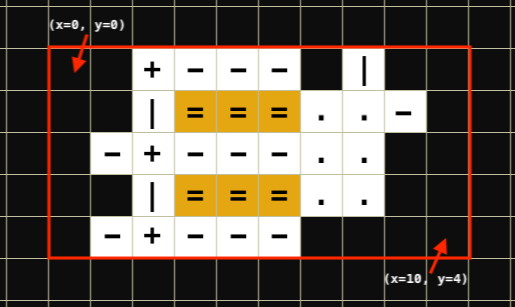
\includegraphics[scale=0.5]{grid.jpg}

  white cells are traversable, black cells are \t{bricks}, yellow cells are \t{woods},
  and the red rectangle is corresponding to the input map.
\end{center}
